\documentclass[a4paper,norsk]{article}
\usepackage{preamble}

\begin{document}
\maketitle
\section*{Operation Swift Trident}
In this section we will asses every step of the marine engineering of operation Swift Trident. It is in our interest to ensure our client expectations of quality and safety are met, and therfore we will take a closer look of each phase of the operation.
\\
Operation Swift Tridents mission is to transport sixteen torpedo anchors from shore to oilfield XM2, execute accurate and safe lifting operations to install these on the seabed. The operation can be divided into .. phases:  
\begin{itemize}
\item Load out
\item Transport
\item Installation 
\end{itemize}

\section*{Load out}
During the first phase we will be located at Marek \textbf{dock 3}, where the torpedo anchors will delivered by our sister company Poseidon.
Thoroughly computations by their engineers have concluded that the TG2 anchor will meet your platform demands.
\\ 
%\begin{SCfigure} %\centering %\caption{Units: 16 Weigth \\ 50 tons \\Front area1 1:5} %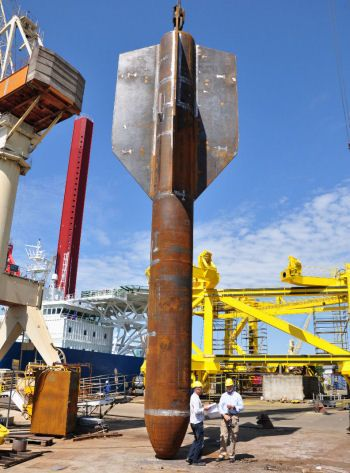
\includegraphics[width=0.3\textwidth]{tt2.jpg}
%\end{SCfigure}
\begin{wrapfigure}{r}{0.5\textwidth}
  \vspace{-20pt}
  \begin{center}
    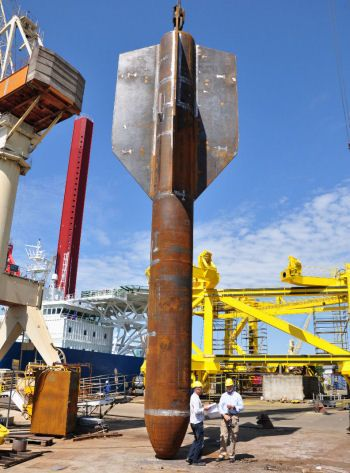
\includegraphics[width=0.25\textwidth]{tt2.jpg}
  \end{center} 
  \vspace{-20pt}
  \caption{TG2 anchor}
  \vspace{-10pt}
\end{wrapfigure}
\textbf{Units}: 16  \\ \\ \textbf{Weigth}: 50 tons \\ \\  \textbf{Frontal area}: 1:5 $m^2$
\\ \\ \\ \\ \\ \\ \\ \\ \\ \\ 
Several factors  has to be evaluated to ensure the safety of personell and equipment, and smooth and time efficient execution.
\subsection*{Weather}
The load out phase is from a weather point of view, only confined by strong winds. Dock 3 is located behind the harbours breakwater modules, meaning sea conditions will have no impact on this phase of the operation. Due to the design of the torpedo, strong winds can have an effect on the rear end of the module, making it twist during the load out on to the vessel for transport. Due to the weight of the anchors this effect will be limited, but will be controlled simply by ropes to make sure it holds prefered angle relative to the vessel upon loading.
\subsection*{Personell Controll}
Both Dock 3 and the loading deck of the vessel will be crowded of personell, therefore strict operation procedures must be implemented to ensure staff safety. Especially during the lifting we have risk of damage, if these procedures are not followed. 

\begin{itemize}
\item Lifting lanes will be established to controll the route of the anchors on the vessel, and NOGO zones to keep personell outside lane area during the lift.  
\item Designated areas for each section of personell with teamleaders, maintaining control of personell so no sections interfere with each other. 
\item Communication with radios between teamleaders and operation chief, to ensure situational awareness and fast response time to sudden changes during lift. 
\end{itemize}

\subsection*{Vessel and Securing}

For this operation we will use a offshore construction vessel UT 790 WP, delivered by Rolls-Royce. It's a modern and well equiped vessel for offshore and subsea operations. The vessel features \\
\begin{wrapfigure}{r}{0.5\textwidth}
  \vspace{-20pt}
  \begin{center}
    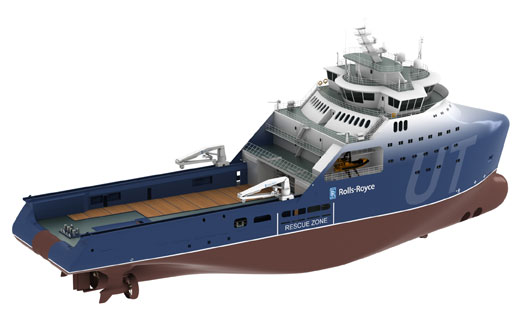
\includegraphics[width=0.4\textwidth]{wessel.jpg}
  \end{center} 
  \vspace{-20pt}
  \caption{ST-261 vessel}
  \vspace{-10pt}
\end{wrapfigure}


\begin{itemize}
\item Main engines: 4x 2765 kW
\item Bollard pull: 270 tonns
\item Supports chain operations down to 2,000 m
\item Buoyancy in the cargo railings for good stability
\item ROV operations
\item Dynamic positioning system 
\end{itemize}
The UT 790 WP is specially equipped for anchor deployment operations. Upon load-out the anchors will be tightly secured with chain. They will be positioned 3 anchors on each side of the deck, with one ready in the skid position for deployment. 
Due too the 
number of anchors to be deployed, two trips to  oilfield XM2 must be maid with half of the anchors each time.

\newpage
\section*{Transportation}

The Rolls-Royce Safer Deck Operations is a system of procedures and equipment ment to ensure personell safety and operational efficiency. The core concept is to reduce personell on deck during achoring operations using cranes at each side of the vessel on a base of rails. These are controlled by certified personel in vantage positions using mobile joysticks. Several splints and other control measures such as "shark jaws "  ensures equipment stays in place during transportation. \\
The vessel itself is though and can handle harsh weather due to its front design ment to pierce the waves rather than riding them. This ensures more stability onboard as well as comfort for onboard personell. Test results have shown the vessel can handle waves up to 9 meters without seawater above forecastle deck level. Even though this is a safe wessel, there are some conditions to adress to make the trip safe for personell and equipment.     
\subsection*{Weather}
Due to its well designed hull, wave conditions must be rahter extreme to halt this phase of the operation when it comes to the ship. The weakness lies in the chain securing the torpedo anchors on board, which will during though weather exposed to significant strain. Our engineer department have used quality computational software to take a look at several worst case scenarios to conclude under what circumstances the transport phase is at risk. This analysis consist mainly of hydrodynamic and chain strain analyses, to assert how the vessel and load will interact during harsh weather conditions. Through logical and obvious precautions such as these, we to a certain degree what kind of worst case scenarios we might encounter and how to access these conditions. 

\subsection*{Securing}
Due to the state of the art of Rolls-Royce Safer Deck Operations, several precautions are made to ensure cargo stays on its assigned deckposition during transport. All anchors are tightly secured to deck with chain, able to withstand strain well over maximum weather conditions which we are comfortable to continue operations. This part of the operation has in offshore history come with a lot of risk due to personell handling wires and chains under high tension. This is now reduced due to new procedures and mentioned remotely controlled cranes, which can do most of the dangerous work.\\
During transport assigned personell will monitor the deck and take inspection rounds, ensuring anchors are tightly locked to the vessel as well as checking that all operational and securing equipment is free for damages and fully working. 

\newpage
\section*{Deploying}
When UT 790 WP has reached oilfield XM2, we commence the final phase of the operation. During transport, weather conditions play an important role deciding when the operation is within safety conditions. Extreme conditions under this final phase are also simulated with modern high quality simulations, resulting in a well established overview of when we can ensure a quality and efficient execution as well as safety for the crew. What we are looking at in these analysis are mainly to identify hydrodynamic forces on the vessel and acceleration of the anchors due to:
\begin{itemize}
\item Object slamming
\item Wave-vessel interaction
\item Crane operation motions
\end{itemize}

\begin{wrapfigure}{r}{0.5\textwidth}
  \vspace{-60pt}
  \begin{center}
    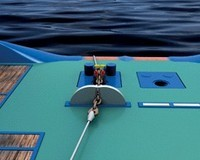
\includegraphics[width=0.4\textwidth]{sharkjaw.jpg}
  \end{center} 
  \vspace{-20pt}
  \caption{Sharkjaw}
  \vspace{-10pt}
\end{wrapfigure}

 One of the reasons of choosing UT 790 WP is reducing crane operations during deployment of the anchors. The main reason for this is that the risk of slamming during cranelift in high waves is no longer a factor, because the anchors will be deployed from deck aft of the vessel.   Shark jaws will hold the anchors in place until we are on the assigned location for the drop for better safety and accurate drop. All these factors will mean safer handeling during harsh conditions. The UT 790 WP is equipped with dynamic positioning system, enabling the vessel to hold a coordinate location with high accuracy using its own propellers, rather than relying on additional anchoring system.
\\ \\ \\ \\ 
Ofcourse bad weather combined with high waves can make this phase of the operation go slower. With significant wave-vessel simulation and analysis, we know our limits and when we can execute a quality and efficient deployment.  
\\
During our last meeting there was some scepticism arising from your side, questioning resonance in the wire and if the torpedo-anchor will reach its desired velocity prior to impact with the sea floor. We would like to adress your uncertainty in this section to make sure everyone is comfortable with how we have adressed problem, and that the risk of failure is at its minimum. 
\\
So lets get a overview of the factors to make a simple calculation to show we are not violating the terms of success. First lets adress the concern if the torpedo-anchors will reach their critical velocity 50 m/s. We can show this is feasible by showing that the free fall velocity is higher in the water. First let us define some values which have an effect in the calculations.
\begin{itemize}
\item The added mass of the anchor $m_a$ 
\item The density of water $\rho$
\item The dimensionless drag coefficient $C_d$
\item The frontal area S
\end{itemize}

 Assuming that the attached wire to the anchor doesn't effect the free fall, newtons second law gives us the following relation.

\begin{align}
(m+m_a)\textbf{a} = \frac{1}{2}\rho SC_d \textbf{V}^2 - m\textbf{g}
\end{align}

Where the first part on the left hand side is a model for viscous drag, and the second is the acceleration of gravity. Using a simple numerical approach we have produced the following result.
\newpage
\begin{figure}[h!]
\centering
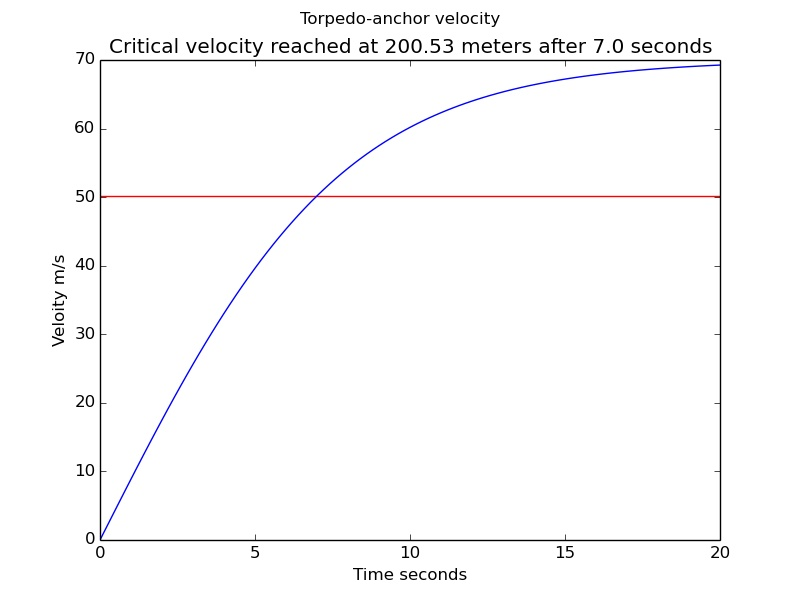
\includegraphics[width=0.6\textwidth]{velocity.jpg}
\end{figure}
In our area of operation the final depth of deployment is at 300 meters. From our calculations we can conclude that the operation is safely within conditions of success, by observing that the desired velocity of 50 m/s achieved at 200 meters.
\\
Following up on the second concern, firstly crane operations are reduced to a minimum because of the deployment of anchors happens at the aft of the vessel, not with a cranelift. Even though, lets say we have a problem during the deployment leaving the anchor at 30 meters. Using the given value of the wire stiffness we can calculate the resonance

\begin{align}
k = \frac{EA}{L} &= \frac{200 000 *10^3 N}{30 m} = 6666666.67 N/m \\
f &= \frac{1}{2\pi} \sqrt{\frac{k}{m}} = \frac{1}{2\pi} \sqrt{\frac{6666666.67 N/m}{50000 Kg}} = \frac{1.83}{s}
\end{align}
At sea a frequency of $1.83s^{-1}$ is not a typical wavecondition at sea, at least not in storms and bad weather. Even though if the wire got stuck and the anchor was hanning close to the sea bed, the frequency would not be low enough to raise any danger.
\\
With this we conclude this appendix of operation Swift Trident. We hope this overview have given new insight and overview of the whole process of getting the torpedo-anchors from shore to the assigned location. If you have any questions do not hesitate to contact us.


\end{document}